%!TEX root = ../Kochbuch.tex

% Complete recipe example
\begin{recipe}{Gurkensalat}
    \graph{
        big=pic/gurkensalat,
        small=pic/gurke,
    }
    
    % \introduction{%
    % ``Das ist vergleichsweise einfach, aber man muss viel schneiden.''\flushright --- \emph{Jack the Ripper}
    % }
    
    \ingredients{%
        5 Stück & Gurken\\
        0,5 Bund & Dill\\
        250 g & Joghurt
    }
    
    \preparation{%
        \step Gurken schälen und/oder waschen.
        ~\\
        
        \step Kleinschneiden.
        ~\\
        
        
        \step Dill hacken.
        ~\\
        
        
        \step Alles mit dem Joghurt zusammenkippen, salzen und pfeffern.
        ~\\
        
        
        \step Noch Fragen? Dann lasst es Euch schmecken!
        ~\\[1cm] 
        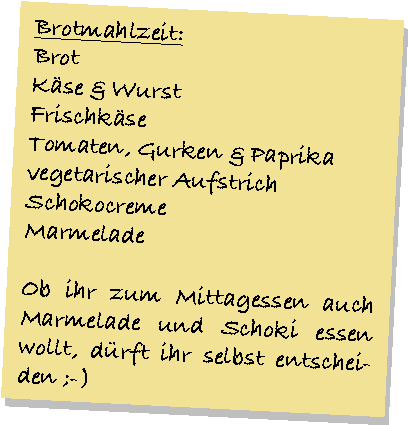
\includegraphics[center,clip=true]{note-brotmahlzeit-crop.pdf}
        
    }

    
    % \hint{%
    %     Noch Fragen? Dann lasst es Euch schmecken!
    % }
    
\end{recipe}